%%%%%%%%%%%%  Generated using docx2latex.com  %%%%%%%%%%%%%%

%%%%%%%%%%%%  v2.0.0-beta  %%%%%%%%%%%%%%

\documentclass[12pt]{article}
\usepackage{amsmath}
\usepackage{latexsym}
\usepackage{amsfonts}
\usepackage[normalem]{ulem}
\usepackage{array}
\usepackage{amssymb}
\usepackage{graphicx}
\usepackage[backend=biber,
style=numeric,
sorting=none,
isbn=false,
doi=false,
url=false,
]{biblatex}\addbibresource{bibliography.bib}

\usepackage{subfig}
\usepackage{wrapfig}
\usepackage{wasysym}
\usepackage{enumitem}
\usepackage{adjustbox}
\usepackage{ragged2e}
\usepackage[svgnames,table]{xcolor}
\usepackage{tikz}
\usepackage{longtable}
\usepackage{changepage}
\usepackage{setspace}
\usepackage{hhline}
\usepackage{multicol}
\usepackage{tabto}
\usepackage{float}
\usepackage{multirow}
\usepackage{makecell}
\usepackage{fancyhdr}
\usepackage[toc,page]{appendix}
\usepackage[hidelinks]{hyperref}
\usetikzlibrary{shapes.symbols,shapes.geometric,shadows,arrows.meta}
\tikzset{>={Latex[width=1.5mm,length=2mm]}}
\usepackage{flowchart}\usepackage[paperheight=11.0in,paperwidth=8.5in,left=1.0in,right=1.0in,top=0.75in,bottom=0.75in,headheight=1in]{geometry}
\usepackage[utf8]{inputenc}
\usepackage[T1]{fontenc}
\TabPositions{0.5in,1.0in,1.5in,2.0in,2.5in,3.0in,3.5in,4.0in,4.5in,5.0in,5.5in,6.0in,}

\urlstyle{same}


 %%%%%%%%%%%%  Set Depths for Sections  %%%%%%%%%%%%%%

% 1) Section
% 1.1) SubSection
% 1.1.1) SubSubSection
% 1.1.1.1) Paragraph
% 1.1.1.1.1) Subparagraph


\setcounter{tocdepth}{5}
\setcounter{secnumdepth}{5}


 %%%%%%%%%%%%  Set Depths for Nested Lists created by \begin{enumerate}  %%%%%%%%%%%%%%


\setlistdepth{9}
\renewlist{enumerate}{enumerate}{9}
		\setlist[enumerate,1]{label=\arabic*)}
		\setlist[enumerate,2]{label=\alph*)}
		\setlist[enumerate,3]{label=(\roman*)}
		\setlist[enumerate,4]{label=(\arabic*)}
		\setlist[enumerate,5]{label=(\Alph*)}
		\setlist[enumerate,6]{label=(\Roman*)}
		\setlist[enumerate,7]{label=\arabic*}
		\setlist[enumerate,8]{label=\alph*}
		\setlist[enumerate,9]{label=\roman*}

\renewlist{itemize}{itemize}{9}
		\setlist[itemize]{label=$\cdot$}
		\setlist[itemize,1]{label=\textbullet}
		\setlist[itemize,2]{label=$\circ$}
		\setlist[itemize,3]{label=$\ast$}
		\setlist[itemize,4]{label=$\dagger$}
		\setlist[itemize,5]{label=$\triangleright$}
		\setlist[itemize,6]{label=$\bigstar$}
		\setlist[itemize,7]{label=$\blacklozenge$}
		\setlist[itemize,8]{label=$\prime$}



 %%%%%%%%%%%%  Header here  %%%%%%%%%%%%%%


\pagestyle{fancy}
\fancyhf{}
\chead{ \chapter{\  }

%%%%%%%%%%%%%%%%%%%% Figure/Image No: 1 starts here %%%%%%%%%%%%%%%%%%%%

\begin{figure}[H]
	\begin{Center}
		\includegraphics[width=6.47in,height=0.11in]{./theme/theme1.xml}
	\end{Center}
\end{figure}


%%%%%%%%%%%%%%%%%%%% Figure/Image No: 1 Ends here %%%%%%%%%%%%%%%%%%%%

\setlength{\parskip}{9.96pt}
}
\cfoot{ 
\vspace{\baselineskip}
\setlength{\parskip}{12pt}
}
\renewcommand{\headrulewidth}{0pt}
\setlength{\topsep}{0pt}\setlength{\parindent}{0pt}

 %%%%%%%%%%%%  This sets linespacing (verticle gap between Lines) Default=1 %%%%%%%%%%%%%%


\renewcommand{\arraystretch}{1.3}


%%%%%%%%%%%%%%%%%%%% Document code starts here %%%%%%%%%%%%%%%%%%%%



\begin{document}


%%%%%%%%%%%%%%%%%%%% Figure/Image No: 2 starts here %%%%%%%%%%%%%%%%%%%%

\begin{figure}[H]
	\begin{Center}
		
\includegraphics[width=6.47in,height=0.11in]{./media/image13.png}
	\end{Center}
\end{figure}


%%%%%%%%%%%%%%%%%%%% Figure/Image No: 2 Ends here %%%%%%%%%%%%%%%%%%%%

\subsection*{ }
\addcontentsline{toc}{subsection}{ }


%%%%%%%%%%%%%%%%%%%% Figure/Image No: 3 starts here %%%%%%%%%%%%%%%%%%%%

\begin{figure}[H]
	\begin{Center}
		
\includegraphics[width=6.46in,height=4.31in]{./media/image18.jpg}
	\end{Center}
\end{figure}


%%%%%%%%%%%%%%%%%%%% Figure/Image No: 3 Ends here %%%%%%%%%%%%%%%%%%%%

\par

\chapter{07.08.2019}\par

\begin{justify}
{\fontsize{18pt}{21.6pt}\selectfont \textbf{Artificial Intelligence Course Assignment}\par}
\end{justify}\par

\begin{justify}
{\fontsize{16pt}{19.2pt}\selectfont \textcolor[HTML]{008575}{Dănciulescu Theodora-Ioana}\par}
\end{justify}\par

\begin{justify}
{\fontsize{14pt}{16.8pt}\selectfont 2nd Year, Group 2.1A\par}
\end{justify}\par

\begin{justify}
{\fontsize{14pt}{16.8pt}\selectfont CE\par}
\end{justify}\par


\vspace{\baselineskip}

\vspace{\baselineskip}

\vspace{\baselineskip}
\section*{Hash function for choosing problem}
\addcontentsline{toc}{section}{Hash function for choosing problem}


%%%%%%%%%%%%%%%%%%%% Figure/Image No: 4 starts here %%%%%%%%%%%%%%%%%%%%

\begin{figure}[H]
\advance\leftskip 0.02in		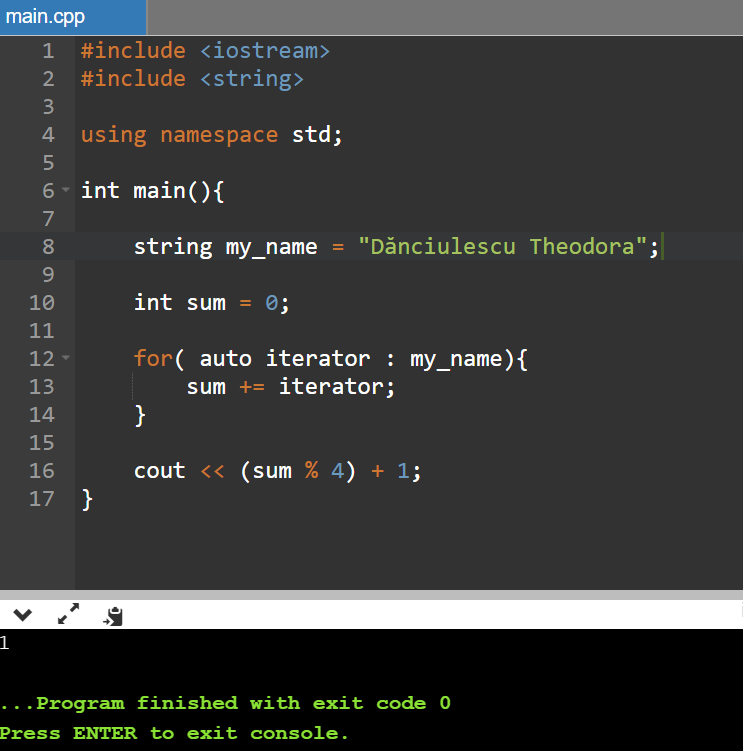
\includegraphics[width=4.29in,height=4.32in]{./media/image11.png}
\end{figure}


%%%%%%%%%%%%%%%%%%%% Figure/Image No: 4 Ends here %%%%%%%%%%%%%%%%%%%%

\begin{justify}
In order to find which problem is assigned to me I had to compute a program that calculates the sum of the ascii codes of the letters in my family name and first name. The simple method of doing this is to simply iterate through the string that represents my name as described above, and adding the ascii code of each character to an integer, called ‘sum’. After iterating through the whole string, the number of the problem will be obtained by the formula: (sum $\%$  4) + 1. A code snippet of the is attached below:
\end{justify}\par


\vspace{\baselineskip}
\begin{justify}
In conclusion, the problem I had to solve was the problem with number 1.
\end{justify}\par


\vspace{\baselineskip}

\vspace{\baselineskip}

\vspace{\baselineskip}
\section*{Problem Statement}
\addcontentsline{toc}{section}{Problem Statement}
\begin{justify}
The statement is presenting the problem of two friends living in Romania in different cities. 
\end{justify}\par


\vspace{\baselineskip}
\begin{justify}
The\ two\ friends want to see each other as soon as possible in a specific city. That’s why they need a software developer to provide each of them the shortest path in distance and also in time. The distance between any two cities is also representing the time required to traverse the road between the two cities.   \tab \tab \tab \tab \tab \tab \tab 
\end{justify}\par


\vspace{\baselineskip}
\begin{justify}
Given\ the map of Romania and the road distances between the cities, an optimum path has to be computed for each friend in order to reach the established destination. Also, beside the optimum path,  they would like to know how much the first arrived friend would have to wait for the other one if they leave their home cities simultaneously.\tab \tab \tab 
\end{justify}\par


\vspace{\baselineskip}
\begin{justify}
In order to proceed with these actions there will be set:\tab 
\end{justify}\par

\tab \tab \tab \tab 
\vspace{\baselineskip}\begin{justify}
Initial\_state: $ \{ $ eg: Sibiu$ \} $ \tab \tab \tab \tab \tab \tab \tab \tab \tab Goal\_state: $ \{ $ eg.Bucharest$ \} $ \tab \tab \tab \tab \tab \tab \tab \tab \tab \tab Path: [‘Rimnicu’, ‘Pitesti’, ‘Bucharest’]\tab \tab \tab \tab \tab \tab \tab \tab Cost: 278
\end{justify}\par

\section*{Problem approach}
\addcontentsline{toc}{section}{Problem approach}
\subsection*{1.\hspace*{10pt}Programming Language}
\addcontentsline{toc}{subsection}{1.\hspace*{10pt}Programming Language}
\begin{adjustwidth}{0.5in}{0.0in}
\begin{justify}
I\ chose to implement the problem in Python because it is a popular language in the domain of Artificial Intelligence.  Also, I like coding in Python for the implementation simplicity, the variety of default functions, the easy way of declaring and managing complicated data structures. Another reason for choosing Python was for adapting the laboratory framework to my problem easily.
\end{justify}\par

\end{adjustwidth}

\subsection*{2.\hspace*{10pt}Search algorithm strategy}
\addcontentsline{toc}{subsection}{2.\hspace*{10pt}Search algorithm strategy}
\begin{adjustwidth}{0.5in}{0.0in}
\begin{justify}
The key idea for an optimal solution with respect to the usage of memory and also the time performance includes a heuristic search algorithm. 
\end{justify}\par

\end{adjustwidth}

\begin{adjustwidth}{0.5in}{0.0in}
\begin{justify}
\textcolor[HTML]{555555}{\parbox{\linewidth}{The A$\ast$  Search algorithm performs better than the Dijkstra’s algorithm because of its use of }}\textbf{heuristics.}}}
\end{justify}\par

\end{adjustwidth}

\begin{adjustwidth}{0.5in}{0.0in}
\begin{justify}
\textcolor[HTML]{555555}{\parbox{\linewidth}{The cities of the romanian map will represent the nodes in an undirected graph, and the distances between the cities will represent the cost of the edges. Using the A$\ast$  search strategy the a path from a given city will be computed to the goal city. The correctitude of the result will be checked performing Dikstra’s algorithm on the same graph. }}}
\end{justify}\par

\end{adjustwidth}


\vspace{\baselineskip}
\section*{Modules}
\addcontentsline{toc}{section}{Modules}

\vspace{\baselineskip}
\begin{justify}
The application contains 7 modules that contributes to a good organisation of the application’s functionality. In order to solve the problem using heuristic search strategy there will be used a set of self-defined classes for defining the problem, these classes were also used at the laboratory sessions for solving other AI problems. These classes will be defined in a separate module. The specific class for our problem is a class inherited from the base class ‘Problem’. Several function will be overwritten in order to obtain the right functionality.
\end{justify}\par


\vspace{\baselineskip}
\begin{justify}
Using the classes used in the laboratory framework: ‘Problem’, ‘Node’, ‘PriorityQueue’ and other functions such like ‘best\_first\_graph\_search’, ‘memoize’, ‘astar\_search’ the solution of the given problem will be computed.
\end{justify}\par

\begin{justify}
Inheriting from the base general class ‘Problem’, I created the ‘FriendsMeetingProblem’ ( this class is created based on the skeleton of the ‘GraphProblem’ class from the laboratory framework) class that will generate an initial\_state, goal\_state(destination) also it contains functions for generating the possible\_actions. In our case the possible\_actions of a certain state represents the adjacent nodes of the current node. Also, the function that generates the result of a given state will return nothing else than the neighbour of that node.
\end{justify}\par

\begin{justify}
The purpose of this application is to compute an optimal path regarding the cost of the path for each of the two friends. 
\end{justify}\par

\subsection*{Input/Output example}
\addcontentsline{toc}{subsection}{Input/Output example}
\subsubsection*{\hspace*{10pt}Input}
\addcontentsline{toc}{subsubsection}{\hspace*{10pt}Input}
\begin{justify}
\tab The input is represented by 3 cities with the following meanings:
\end{justify}\par

\begin{justify}
\tab City1 - the initial state of friend A
\end{justify}\par

\begin{justify}
\tab City2 - the initial state of friend B
\end{justify}\par

\begin{justify}
\tab City3 - the meeting point of the 2 friend
\end{justify}\par

\begin{justify}
The input is randomly generated by one of the program modules. 
\end{justify}\par

\begin{justify}
\tab Take the following input:
\end{justify}\par

\begin{justify}
\tab City1 <- Fagaras
\end{justify}\par

\begin{justify}
\tab City2 <- Oradea
\end{justify}\par

\begin{justify}
\tab City <- Eforie
\end{justify}\par

\subsubsection*{Output}
\addcontentsline{toc}{subsubsection}{Output}
\begin{adjustwidth}{0.5in}{0.0in}
\begin{justify}
The output is designated to:
\end{justify}\par

\end{adjustwidth}

\begin{adjustwidth}{0.5in}{0.0in}
\begin{justify}
- display the solution path of every friend
\end{justify}\par

\end{adjustwidth}

\begin{adjustwidth}{0.5in}{0.0in}
\begin{justify}
- display the initial data of the problem 
\end{justify}\par

\end{adjustwidth}

\begin{adjustwidth}{0.5in}{0.0in}
\begin{justify}
- display if the found path is the correct one (verIfied with Dikstra’s algorithm) 
\end{justify}\par

\end{adjustwidth}

\begin{adjustwidth}{0.5in}{0.0in}
\begin{justify}
- display the amount of time the first arrived friend will wait for the other one
\end{justify}\par

\end{adjustwidth}

\begin{adjustwidth}{0.5in}{0.0in}
\begin{justify}
- display an execution time analysis of the program
\end{justify}\par

\end{adjustwidth}



%%%%%%%%%%%%%%%%%%%% Figure/Image No: 5 starts here %%%%%%%%%%%%%%%%%%%%

\begin{figure}[H]
\advance\leftskip 0.62in		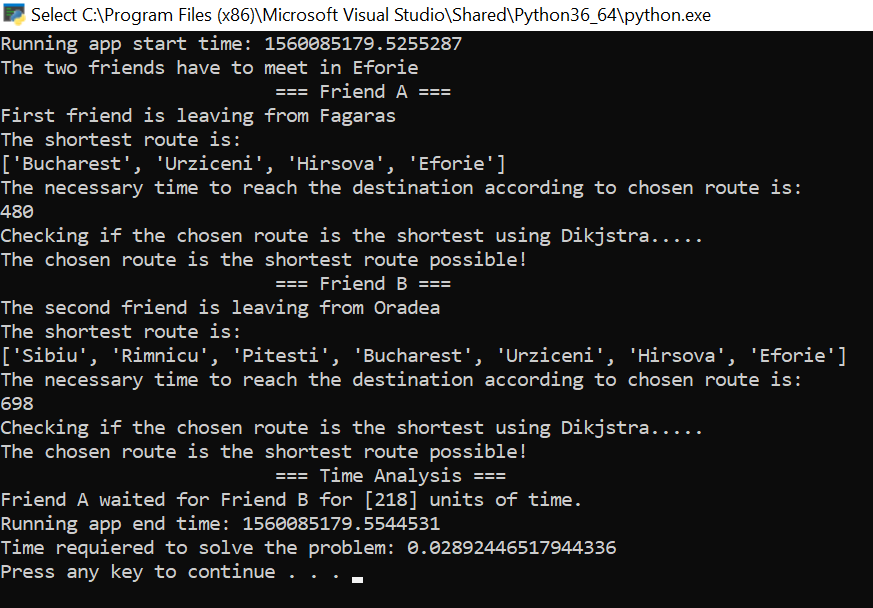
\includegraphics[width=5.86in,height=4.09in]{./media/image1.png}
\end{figure}


%%%%%%%%%%%%%%%%%%%% Figure/Image No: 5 Ends here %%%%%%%%%%%%%%%%%%%%

\par

\begin{justify}
A brief description of every module and the pseudocode for the new functions added by me are presented below:
\end{justify}\par


\vspace{\baselineskip}
\subsection*{1.\hspace*{10pt}RomaniaMapBuild.py}
\addcontentsline{toc}{subsection}{1.\hspace*{10pt}RomaniaMapBuild.py}
\begin{adjustwidth}{0.5in}{0.0in}
\begin{justify}
This\ module contains the data structures containing data about the Romania map.  These data structures are used globally in the application as the Romania map data is constant. 
\end{justify}\par

\end{adjustwidth}

\begin{adjustwidth}{0.5in}{0.0in}
\begin{justify}
More precisely, contains the following: 
\end{justify}\par

\end{adjustwidth}

\begin{adjustwidth}{0.5in}{0.0in}
\begin{justify}
-a\ list with unique occurrences of  all the cities
\end{justify}\par

\end{adjustwidth}

\begin{adjustwidth}{0.5in}{0.0in}
\begin{justify}
 -a dictionary that represents the adjacency list of the graph represented by the links between the cities from Romania with the correspondent costs
\end{justify}\par

\end{adjustwidth}

\begin{adjustwidth}{0.5in}{0.0in}
\begin{justify}
-a dictionary with the plane coordinates of every city.
\end{justify}\par

\end{adjustwidth}

\begin{adjustwidth}{0.5in}{0.0in}
\begin{justify}
-Node instances of the cities are created for further implementation simplicity.
\end{justify}\par

\end{adjustwidth}

\subsubsection*{\hspace*{10pt}Data structures used}
\addcontentsline{toc}{subsubsection}{\hspace*{10pt}Data structures used}
\begin{itemize}
	\item \textbf{romania\_map[start\_city][destination\_city]=road\_cost }: adjacency dictionary of the roads between the cities(nodes) represents keys and the cost between the two cities as the value.\par

	\item \textbf{romania\_map\_coordinates[city] = ( x, y) }: dictionary with the XOY coordinates of every city in the scaled map\par

	\item \textbf{city\_list }: list with unique Node instances of the cities.
\end{itemize}\par


\vspace{\baselineskip}

\vspace{\baselineskip}
\subsection*{2.\ \ \ \ \ \  input\_generator.py}
\addcontentsline{toc}{subsection}{2.\ \ \ \ \ \  input\_generator.py}
\begin{adjustwidth}{0.5in}{0.0in}
\begin{justify}
This\ module contains a function that randomly chooses the initial\_state of every friend and the meeting point of the two friends. This is done shuffling the list of the Node instances of the cities  and then choosing the three cities with their specific meaning.
\end{justify}\par

\end{adjustwidth}

\begin{adjustwidth}{0.5in}{0.0in}
\begin{justify}
Pseudocode
\end{justify}\par

\end{adjustwidth}

\begin{adjustwidth}{0.5in}{0.0in}
\begin{justify}
{\fontsize{8pt}{9.6pt}\selectfont \textbf{function} input\_generator()\textbf{ returns} tuple of nodes  \tabto{0.75in} \tab \tab \tab \par}
\end{justify}\par

\end{adjustwidth}

\begin{adjustwidth}{0.5in}{0.0in}
\begin{justify}
 \tabto{0.75in} {\fontsize{8pt}{9.6pt}\selectfont \textbf{persistent:}\textit{copy\_city\_list}, copy of list of nodes\par}
\end{justify}\par

\end{adjustwidth}

\begin{adjustwidth}{0.5in}{0.0in}
\begin{justify}
{\fontsize{8pt}{9.6pt}\selectfont  \tabto{0.75in} \ \  \tab \tab in map\par}
\end{justify}\par

\end{adjustwidth}

\begin{adjustwidth}{0.5in}{0.0in}
\begin{justify}
 \tabto{0.75in} \tab \tab {\fontsize{8pt}{9.6pt}\selectfont \textit{start1}, Node instance\par}
\end{justify}\par

\end{adjustwidth}

\begin{adjustwidth}{0.5in}{0.0in}
\begin{justify}
 \tabto{0.75in} \tab \tab {\fontsize{8pt}{9.6pt}\selectfont \textit{start2}, Node instance\par}
\end{justify}\par

\end{adjustwidth}

\begin{adjustwidth}{0.5in}{0.0in}
\begin{justify}
{\fontsize{8pt}{9.6pt}\selectfont  \tabto{0.75in} \tab \tab destination,Node instance\par}
\end{justify}\par

\end{adjustwidth}

\begin{adjustwidth}{0.5in}{0.0in}
\begin{justify}
{\fontsize{8pt}{9.6pt}\selectfont  \tabto{0.75in} copy\_city\_list <- city\_list\par}
\end{justify}\par

\end{adjustwidth}

\begin{adjustwidth}{0.5in}{0.0in}
\begin{justify}
{\fontsize{8pt}{9.6pt}\selectfont  \tabto{0.75in} shuffle(copy\_city\_list)\par}
\end{justify}\par

\end{adjustwidth}

\begin{adjustwidth}{0.5in}{0.0in}
\begin{justify}
 \tabto{0.75in} {\fontsize{8pt}{9.6pt}\selectfont \textbf{returns}\ (start1,\ start2,\ destination)    \par}
\end{justify}\par

\end{adjustwidth}

\subsection*{3.\hspace*{10pt}test\_module.py}
\addcontentsline{toc}{subsection}{3.\hspace*{10pt}test\_module.py}
\begin{adjustwidth}{0.5in}{0.0in}
\begin{justify}
This module contains the function that verifies the result computed by the A$\ast$  search with the result computed by the Dijkstra’s algorithm. The functions used:
\end{justify}\par

\end{adjustwidth}

\begin{itemize}
	\item dijkstra(start\_node, end\_node) -\textcolor[HTML]{999999}{ }Dijkstra’s shortest path algorithm is\textcolor[HTML]{666666}{ an algorithm for finding the shortest paths between nodes in a graph, which may represent, for example, road networks.\ This algorithm guarantees to find the shortest path between any 2 given nodes in  \( $ \{ $ $\textbackslash$ displaystyle O($ \vert $ E$ \vert $ +$ \vert $ V$ \vert $ $\textbackslash$ log $ \vert $ V$ \vert $ )$ \} $  }}{\fontsize{10pt}{12.0pt}\selectfont \textcolor[HTML]{666666}{(where $ \{ $ $\textbackslash$ displaystyle $ \vert $ E$ \vert $ $ \} $  \)\par} is the number of edges) as it is implemented using a min PriorityQueue.}}\par

\begin{itemize}
	\item \textcolor[HTML]{666666}{\parbox{\linewidth}{Functionality : This function returns the minimum path cost computed with Dijkstra’s from start\_node to end\_node. }}}\par

	\item \textcolor[HTML]{666666}{Parameters:}}
\end{itemize}\par

\begin{adjustwidth}{1.5in}{0.0in}
\begin{justify}
\textcolor[HTML]{666666}{\parbox{\linewidth}{-start\_node : source Node instance, the function will find all the minimum paths from this node to all the other nodes.}}}
\end{justify}\par

\end{adjustwidth}

\begin{adjustwidth}{1.5in}{0.0in}
\begin{justify}
\textcolor[HTML]{666666}{\parbox{\linewidth}{-end\_node : the Node instance that we are interested in finding the shortest path to reach it }}}
\end{justify}\par

\end{adjustwidth}

\begin{itemize}
	\item \textcolor[HTML]{666666}{Return value: the return value is an integer representing the minimum }}
\end{itemize}\par

\begin{justify}
\textcolor[HTML]{666666}{\  \tab \tab \tab \ path cost from the  start\_node to the end\_node.}}
\end{justify}\par

	\item \textcolor[HTML]{666666}{\parbox{\linewidth}{test\_function(astar\_cost, start\_node, end\_node) - this function return a bool that verifies if the cost computed by the A$\ast$  search is identical with the cost computed by Dikjstra’s algorithm.}}}
\end{itemize}\par

\begin{itemize}
	\item \textcolor[HTML]{666666}{\parbox{\linewidth}{Functionality: compares the cost generated by A$\ast$  search with the cost generated by Dijkstra’s algorithm.}}}\par

	\item \textcolor[HTML]{666666}{Parameters:}}
\end{itemize}\par

\begin{adjustwidth}{1.5in}{0.0in}
\begin{justify}
\textcolor[HTML]{666666}{- astar\_cost: cost resulted from the A$\ast$  search}}
\end{justify}\par

\end{adjustwidth}

\begin{adjustwidth}{1.5in}{0.0in}
\begin{justify}
\textcolor[HTML]{666666}{\parbox{\linewidth}{-start\_node : source Node instance, the function will find all the minimum paths from this node to all the other nodes.}}}
\end{justify}\par

\end{adjustwidth}

\begin{adjustwidth}{1.5in}{0.0in}
\begin{justify}
\textcolor[HTML]{666666}{\parbox{\linewidth}{-end\_node : the Node instance that we are interested in finding the shortest path to reach it }}}
\end{justify}\par

\end{adjustwidth}

\begin{itemize}
	\item \textcolor[HTML]{666666}{Return value: the returned value is a boolean that points out if the}}
\end{itemize}\par

\begin{adjustwidth}{1.0in}{0.0in}
\begin{justify}
\textcolor[HTML]{666666}{result computed using heuristic search strategy is correct or not. }}
\end{justify}\par

\end{adjustwidth}


\vspace{\baselineskip}

\vspace{\baselineskip}

\vspace{\baselineskip}
\tab 
\vspace{\baselineskip}\begin{justify}
{\fontsize{14pt}{16.8pt}\selectfont Pseudocode\par}
\end{justify}\par

\begin{adjustwidth}{0.5in}{0.0in}
\begin{justify}
{\fontsize{8pt}{9.6pt}\selectfont \textbf{function }dijkstra(start\_node, end\_node) \textbf{returns} of integer  \tabto{0.75in} \tab \tab \tab \tab \tab \textbf{persistent}:\textit{distances,}dictionary of distances from start\_node to all the other cities\par}
\end{justify}\par

\end{adjustwidth}

\begin{adjustwidth}{0.5in}{0.0in}
\begin{justify}
 \tabto{0.75in} \tab \tab {\fontsize{8pt}{9.6pt}\selectfont \textit{q},default min priority queue of pairs of \par}
\end{justify}\par

\end{adjustwidth}

\begin{adjustwidth}{0.5in}{0.0in}
\begin{justify}
{\fontsize{8pt}{9.6pt}\selectfont  \tabto{0.75in} \tab \tab (cost, destination)\par}
\end{justify}\par

\end{adjustwidth}

\begin{adjustwidth}{0.5in}{0.0in}
\begin{justify}
 \tabto{0.75in} \tab {\fontsize{8pt}{9.6pt}\selectfont \textbf{for} i \textbf{in} city\_list \textbf{do }\par}
\end{justify}\par

\end{adjustwidth}

\begin{adjustwidth}{0.5in}{0.0in}
\begin{justify}
{\fontsize{8pt}{9.6pt}\selectfont  \tabto{0.75in} \tab \tab distances[i] = MAX\_VALUE\par}
\end{justify}\par

\end{adjustwidth}

\begin{justify}
{\fontsize{8pt}{9.6pt}\selectfont  \tabto{0.75in} \tab distances[start\_node] = 0\par}
\end{justify}\par

\begin{justify}
{\fontsize{8pt}{9.6pt}\selectfont  \tabto{0.75in} \tab q.insert(pair(0, start\_node))\par}
\end{justify}\par

\begin{justify}
 \tabto{0.75in} \tab {\fontsize{8pt}{9.6pt}\selectfont \textbf{while} q i\textbf{s not }empty \textbf{do}\par}
\end{justify}\par

\begin{justify}
{\fontsize{8pt}{9.6pt}\selectfont  \tabto{0.75in} \tab \tab current <- q.top()\par}
\end{justify}\par

\begin{justify}
{\fontsize{8pt}{9.6pt}\selectfont  \tabto{0.75in} \tab \tab current\_city <- current[1]\par}
\end{justify}\par

\begin{justify}
 \tabto{0.75in} \tab \tab {\fontsize{8pt}{9.6pt}\selectfont \textbf{for} neighbour \textbf{in} romania\_map[current\_city]\textbf{ do}\par}
\end{justify}\par

\begin{adjustwidth}{0.5in}{0.0in}
\begin{justify}
 \tabto{0.75in} \tab \tab \tab {\fontsize{8pt}{9.6pt}\selectfont \textbf{if} distances[neighbour] > distances[current\_city] + \tab \tab \tab \tab \tab \tab \tab \tab \tab romania\_map[current\_city][neighbour] \textbf{then}\par}
\end{justify}\par

\end{adjustwidth}

\begin{adjustwidth}{0.5in}{0.0in}
\begin{justify}
{\fontsize{8pt}{9.6pt}\selectfont  \tabto{0.75in} \tab \tab \tab \tab distances[neighbour] = distances[current\_city] + \tab \tab \tab \tab \tab \tab \tab \tab \tab romania\_map[current\_city][neighbour]\par}
\end{justify}\par

\end{adjustwidth}

\begin{adjustwidth}{0.5in}{0.0in}
\begin{justify}
{\fontsize{8pt}{9.6pt}\selectfont  \tabto{0.75in} \tab \tab \tab \tab q.insert(pair(distances[neighbour], neighbour))\par}
\end{justify}\par

\end{adjustwidth}

\tab \tab 
\vspace{\baselineskip}\tab \tab \tab \tab 
\vspace{\baselineskip}\begin{adjustwidth}{0.5in}{0.0in}
\begin{justify}
 \tabto{0.75in} \tab {\fontsize{8pt}{9.6pt}\selectfont \textbf{returns }destination[end\_node]\  \par}
\end{justify}\par

\end{adjustwidth}


\vspace{\baselineskip}\begin{adjustwidth}{0.5in}{0.0in}
\begin{justify}
{\fontsize{8pt}{9.6pt}\selectfont \textbf{function }test\_function(astar\_cost, start, destination) returns bool value\par}
\end{justify}\par

\end{adjustwidth}

\begin{justify}
{\fontsize{8pt}{9.6pt}\selectfont \   \tabto{0.75in} \textbf{persistent}:\textit{astar\_cost}, integer representing the cost generated by the astar\par}
\end{justify}\par

\begin{adjustwidth}{0.5in}{0.0in}
\begin{justify}
{\fontsize{8pt}{9.6pt}\selectfont  \tabto{0.75in} \tab \tab solution\par}
\end{justify}\par

\end{adjustwidth}

\begin{adjustwidth}{0.5in}{0.0in}
\begin{justify}
 \tabto{0.75in} \tab \tab {\fontsize{8pt}{9.6pt}\selectfont \textit{start}, Node instance\par}
\end{justify}\par

\end{adjustwidth}

\begin{adjustwidth}{0.5in}{0.0in}
\begin{justify}
{\fontsize{8pt}{9.6pt}\selectfont  \tabto{0.75in} \tab \tab destination,Node instance\tab \tab \tab \tab \par}
\end{justify}\par

\end{adjustwidth}

\begin{adjustwidth}{0.5in}{0.0in}
\begin{justify}
 \tabto{0.75in} {\fontsize{8pt}{9.6pt}\selectfont \textbf{returns }(astar = dijkstra(start, destination)\par}
\end{justify}\par

\end{adjustwidth}


\vspace{\baselineskip}
\vspace{\baselineskip}

\vspace{\baselineskip}
\subsection*{4.\ \ \  \hspace*{10pt}OutputFormat.py}
\addcontentsline{toc}{subsection}{4.\ \ \  \hspace*{10pt}OutputFormat.py}
\begin{adjustwidth}{0.5in}{0.0in}
\begin{justify}
This module’s target is to group the output functionalities into functions that ensures an understandable output for any user. 
\end{justify}\par

\end{adjustwidth}

\begin{itemize}
	\item run\_app(start\_friend1, start\_friend2, meeting\_point) 
\end{itemize}\par

\begin{enumerate}
	\item Functionality: This functions aims to create all the necessary instances for running the application. There will be created two ‘FriendsMeetingProblem’ instances, in order to compute two optimal paths for each friend. Having these 2 instances, the astar\_search function defined in the utils.py module, the same function used in the solving of the NPuzzleProblem, is called on the two created instances. As a result of the A$\ast$  search algorithm the paths of the 2 friends are created, and using more output function calls, the result will be transmitted in the Output Console in a very understandable way of a result. This function is also containing time execution analysis that will be displayed to the user, too.\par

	\item Parameters:\par

\begin{enumerate}
	\item Start\_friend1 -Node instance, initial state node of Friend A\par

	\item Start\_friend2 - Node instance, initial state node of Friend B\par

	\item Meeting\_point - Node instance, meeting node of the 2 friends\tab 
\end{enumerate}
\end{enumerate}\par

\begin{justify}
 
\end{justify}\par

\begin{itemize}
	\item output\_route\_analytics(path, cost)
\end{itemize}\par

\begin{enumerate}
	\item Functionality: To print in a nice way a path and its cost\par

	\item Parameters:\par

\begin{enumerate}
	\item Path : list with strings representing the path of a friend\par

	\item Cost: the cost of the path\par


\vspace{\baselineskip}\begin{itemize}
	\item output\_correctitude\_check(cost\_astar, start, destination)
\end{itemize}\par

\begin{justify}
 \tabto{0.75in} \tab \ \ \ \  a)\tab Functionality: To print in a nice way if the result computed by A$\ast$  \tab \tab \tab \tab search is correct using Dijkstra’s to verify the resulted cost
\end{justify}\par

\begin{justify}
  \tabto{0.75in}  \tab \ \ \ \  b)\tab Parameters:
\end{justify}\par

	\item cost\_astar: integer representing the cost computed by A$\ast$  search\par

	\item start: the initial source node from where to start the path\par

	\item Destination: the target node where the path ends
\end{enumerate}
\end{enumerate}\par


\vspace{\baselineskip}\begin{itemize}
	\item output\_time\_waited(first\_to\_destination,\ second\_to\_destination,  time1, time2) 
\end{itemize}\par

\begin{justify}
 \tabto{0.75in} a)\tab Functionality:\ To print the time the first arrived friend has to wait until the second friend arrives.  
\end{justify}\par

\begin{justify}
 \tabto{0.75in}  b)\tab Parameters:
\end{justify}\par

\begin{itemize}
	\item First\_to\_destination : is string representing either $``$Friend A$"$  or $``$Friend B$"$ , depending on the generated result\par

	\item Second\_to\_destination : is string representing either $``$Friend A$"$  or $``$Friend B$"$ , depending on the generated result\par

	\item Time1: represents the time required for the first arrived friend to traverse the path (the cost of the road)\par

	\item Time2:\  represents the time required for the second arrived friend to traverse the path (the cost of the road)
\end{itemize}\par

\begin{justify}
{\fontsize{14pt}{16.8pt}\selectfont Pseudocode\par}
\end{justify}\par

\begin{adjustwidth}{0.5in}{0.0in}
\begin{justify}
{\fontsize{8pt}{9.6pt}\selectfont \textbf{function} run\_app(start\_friend1, start\_friend2, meeting\_point) \tabto{0.75in} \tab \tab \tab \tab \textbf{persistent:}\textit{start\_friend1}, Node instance\par}
\end{justify}\par

\end{adjustwidth}

\begin{adjustwidth}{0.5in}{0.0in}
\begin{justify}
 \tabto{0.75in} \tab \tab {\fontsize{8pt}{9.6pt}\selectfont \textit{start\_friend2}, Node instance\par}
\end{justify}\par

\end{adjustwidth}

\begin{adjustwidth}{0.5in}{0.0in}
\begin{justify}
 \tabto{0.75in} \tab \tab {\fontsize{8pt}{9.6pt}\selectfont \textit{meeting\_point},Node instance\par}
\end{justify}\par

\end{adjustwidth}


\vspace{\baselineskip}\begin{adjustwidth}{0.5in}{0.0in}
\begin{justify}
 \tabto{0.75in} {\fontsize{8pt}{9.6pt}\selectfont \textbf{print}("The two friends have to meet in " + meeting\_point)\par}
\end{justify}\par

\end{adjustwidth}

\begin{adjustwidth}{0.5in}{0.0in}
\begin{justify}
{\fontsize{8pt}{9.6pt}\selectfont \ \ \  friend1 <- FriendsMeetingProblem(start\_friend1, meeting\_point)\par}
\end{justify}\par

\end{adjustwidth}

\begin{adjustwidth}{0.5in}{0.0in}
\begin{justify}
{\fontsize{8pt}{9.6pt}\selectfont \ \ \  path1 <- astar\_search(friend1).solution()\par}
\end{justify}\par

\end{adjustwidth}

\begin{adjustwidth}{0.5in}{0.0in}
\begin{justify}
{\fontsize{8pt}{9.6pt}\selectfont \ \ \  journey\_time1 <- 0\par}
\end{justify}\par

\end{adjustwidth}

\begin{adjustwidth}{0.5in}{0.0in}
\begin{justify}
{\fontsize{8pt}{9.6pt}\selectfont \ \ \  past <- start\_friend1\par}
\end{justify}\par

\end{adjustwidth}

\begin{adjustwidth}{0.5in}{0.0in}
\begin{justify}
{\fontsize{8pt}{9.6pt}\selectfont \ \ \  \textbf{for} i \textbf{in} path1\textbf{ do}\par}
\end{justify}\par

\end{adjustwidth}

\begin{adjustwidth}{0.5in}{0.0in}
\begin{justify}
{\fontsize{8pt}{9.6pt}\selectfont \ \ \ \ \ \ \  journey\_time1 <- journey\_time1 + romania\_map[past][i]\par}
\end{justify}\par

\end{adjustwidth}

\begin{adjustwidth}{0.5in}{0.0in}
\begin{justify}
{\fontsize{8pt}{9.6pt}\selectfont \ \ \ \ \ \ \  past <- i\par}
\end{justify}\par

\end{adjustwidth}

\begin{adjustwidth}{0.5in}{0.0in}
\begin{justify}
{\fontsize{8pt}{9.6pt}\selectfont \ \ \  \textbf{print}(" === Friend A ===")\par}
\end{justify}\par

\end{adjustwidth}

\begin{adjustwidth}{0.5in}{0.0in}
\begin{justify}
{\fontsize{8pt}{9.6pt}\selectfont \ \  \textbf{ print}("First friend is leaving from " + start\_friend1)\par}
\end{justify}\par

\end{adjustwidth}

\begin{adjustwidth}{0.5in}{0.0in}
\begin{justify}
{\fontsize{8pt}{9.6pt}\selectfont \ \ \  output\_route\_analytics(path1, journey\_time1)\par}
\end{justify}\par

\end{adjustwidth}

\begin{adjustwidth}{0.5in}{0.0in}
\begin{justify}
{\fontsize{8pt}{9.6pt}\selectfont \ \ \  output\_correctitude\_check(journey\_time1, start\_friend1, meeting\_point)\par}
\end{justify}\par

\end{adjustwidth}

\begin{adjustwidth}{0.5in}{0.0in}
\begin{justify}
{\fontsize{8pt}{9.6pt}\selectfont \ \ \  friend2 <- FriendsMeetingProblem(start\_friend2, meeting\_point)\par}
\end{justify}\par

\end{adjustwidth}

\begin{adjustwidth}{0.5in}{0.0in}
\begin{justify}
{\fontsize{8pt}{9.6pt}\selectfont \ \ \  path2 <- astar\_search(friend2).solution()\par}
\end{justify}\par

\end{adjustwidth}

\begin{adjustwidth}{0.5in}{0.0in}
\begin{justify}
{\fontsize{8pt}{9.6pt}\selectfont \ \ \  journey\_time2 <- 0\par}
\end{justify}\par

\end{adjustwidth}

\begin{adjustwidth}{0.5in}{0.0in}
\begin{justify}
{\fontsize{8pt}{9.6pt}\selectfont \ \ \  past <- start\_friend2.state\par}
\end{justify}\par

\end{adjustwidth}

\begin{adjustwidth}{0.5in}{0.0in}
\begin{justify}
{\fontsize{8pt}{9.6pt}\selectfont \ \ \  \textbf{for }i \textbf{in} path2\textbf{ do}\par}
\end{justify}\par

\end{adjustwidth}

\begin{adjustwidth}{0.5in}{0.0in}
\begin{justify}
{\fontsize{8pt}{9.6pt}\selectfont \ \ \ \ \ \ \  journey\_time2 <- journey\_time2 + romania\_map[past][i]\par}
\end{justify}\par

\end{adjustwidth}

\begin{adjustwidth}{0.5in}{0.0in}
\begin{justify}
{\fontsize{8pt}{9.6pt}\selectfont \ \ \ \ \ \ \  past <- i\par}
\end{justify}\par

\end{adjustwidth}

\begin{adjustwidth}{0.5in}{0.0in}
\begin{justify}
{\fontsize{8pt}{9.6pt}\selectfont \ \ \  print(" === Friend B ===")\par}
\end{justify}\par

\end{adjustwidth}

\begin{adjustwidth}{0.5in}{0.0in}
\begin{justify}
{\fontsize{8pt}{9.6pt}\selectfont \ \ \  print("The second friend is leaving from " + start\_friend2)\par}
\end{justify}\par

\end{adjustwidth}

\begin{adjustwidth}{0.5in}{0.0in}
\begin{justify}
{\fontsize{8pt}{9.6pt}\selectfont \ \ \  output\_route\_analytics(path2, journey\_time2)\par}
\end{justify}\par

\end{adjustwidth}

\begin{adjustwidth}{0.5in}{0.0in}
\begin{justify}
{\fontsize{8pt}{9.6pt}\selectfont \ \ \  output\_correctitude\_check(journey\_time2, start\_friend2, meeting\_point)\par}
\end{justify}\par

\end{adjustwidth}

\begin{adjustwidth}{0.5in}{0.0in}
\begin{justify}
{\fontsize{8pt}{9.6pt}\selectfont \ \ \  \textbf{if} journey\_time1 < journey\_time2 \textbf{then}\par}
\end{justify}\par

\end{adjustwidth}

\begin{adjustwidth}{0.5in}{0.0in}
\begin{justify}
{\fontsize{8pt}{9.6pt}\selectfont \ \ \ \ \ \ \  first\_friend <- "Friend A"\par}
\end{justify}\par

\end{adjustwidth}

\begin{adjustwidth}{0.5in}{0.0in}
\begin{justify}
{\fontsize{8pt}{9.6pt}\selectfont \ \ \ \ \ \ \  second\_friend <- "Friend B"\par}
\end{justify}\par

\end{adjustwidth}

\begin{adjustwidth}{0.5in}{0.0in}
\begin{justify}
{\fontsize{8pt}{9.6pt}\selectfont \  \textbf{\  else}\par}
\end{justify}\par

\end{adjustwidth}

\begin{adjustwidth}{0.5in}{0.0in}
\begin{justify}
{\fontsize{8pt}{9.6pt}\selectfont \ \ \ \ \ \ \  first\_friend <- "Friend B"\par}
\end{justify}\par

\end{adjustwidth}

\begin{adjustwidth}{0.5in}{0.0in}
\begin{justify}
{\fontsize{8pt}{9.6pt}\selectfont \ \ \ \ \ \ \  second\_friend <- "Friend A"\par}
\end{justify}\par

\end{adjustwidth}

\begin{adjustwidth}{0.5in}{0.0in}
\begin{justify}
{\fontsize{8pt}{9.6pt}\selectfont \ \ \  output\_time\_waited(first\_friend, second\_friend, journey\_time1, journey\_time2)\par}
\end{justify}\par

\end{adjustwidth}


\vspace{\baselineskip}
\vspace{\baselineskip}\begin{adjustwidth}{0.5in}{0.0in}
\begin{justify}
{\fontsize{8pt}{9.6pt}\selectfont \textbf{function }output\_route\_analytics(path, cost)\par}
\end{justify}\par

\end{adjustwidth}

\begin{justify}
{\fontsize{8pt}{9.6pt}\selectfont \textbf{\ \   \tabto{0.75in} persistent}:\textit{ path}, list with the cities in the path\par}
\end{justify}\par

\begin{adjustwidth}{0.5in}{0.0in}
\begin{justify}
 \tabto{0.75in} \tab \tab {\fontsize{8pt}{9.6pt}\selectfont \textit{cost}, integer as the cost of the path\par}
\end{justify}\par

\end{adjustwidth}

\tab \tab \tab \tab 
\vspace{\baselineskip}\begin{justify}
{\fontsize{8pt}{9.6pt}\selectfont \textbf{ \tabto{0.75in}  print(}"The shortest route is: "\textbf{)}\par}
\end{justify}\par

\begin{justify}
{\fontsize{8pt}{9.6pt}\selectfont \textbf{\ \   \tabto{0.75in}  print(}path\textbf{)}\par}
\end{justify}\par

\begin{justify}
{\fontsize{8pt}{9.6pt}\selectfont \textbf{\ \   \tabto{0.75in}  print(}"The necessary time to reach the destination according to chosen route is: "\textbf{)}\par}
\end{justify}\par

\begin{justify}
{\fontsize{8pt}{9.6pt}\selectfont \textbf{\ \ \   \tabto{0.75in}  print(}cost\textbf{)}\par}
\end{justify}\par


\vspace{\baselineskip}\tab 
\vspace{\baselineskip}\begin{adjustwidth}{0.5in}{0.0in}
\begin{justify}
{\fontsize{8pt}{9.6pt}\selectfont \textbf{function }output\_correctitude\_check(cost\_astar, start, destination)\par}
\end{justify}\par

\end{adjustwidth}

\begin{justify}
{\fontsize{8pt}{9.6pt}\selectfont \textbf{\ \   \tabto{0.75in} persistent}:\textit{ astar\_cost}, integer representing the cost generated by the astar\par}
\end{justify}\par

\begin{adjustwidth}{0.5in}{0.0in}
\begin{justify}
{\fontsize{8pt}{9.6pt}\selectfont  \tabto{0.75in} \tab \tab solution\par}
\end{justify}\par

\end{adjustwidth}

\begin{adjustwidth}{0.5in}{0.0in}
\begin{justify}
 \tabto{0.75in} \tab \tab {\fontsize{8pt}{9.6pt}\selectfont \textit{start}, Node instance\par}
\end{justify}\par

\end{adjustwidth}

\begin{adjustwidth}{0.5in}{0.0in}
\begin{justify}
{\fontsize{8pt}{9.6pt}\selectfont  \tabto{0.75in} \tab \tab destination,Node instance\par}
\end{justify}\par

\end{adjustwidth}

\tab \tab \tab \tab 
\vspace{\baselineskip}\begin{justify}
{\fontsize{8pt}{9.6pt}\selectfont \textbf{ \tabto{0.75in} print(}"Checking if the chosen route is the shortest using Dikjstra....."\textbf{)}\par}
\end{justify}\par

\begin{justify}
{\fontsize{8pt}{9.6pt}\selectfont \textbf{\ \ \   \tabto{0.75in} if }test\_function(cost\_astar, start, destination) = 1\textbf{ then}\par}
\end{justify}\par

\begin{justify}
{\fontsize{8pt}{9.6pt}\selectfont \textbf{\ \ \ \ \ \   \tabto{0.75in} \tab  print(}"The chosen route is the shortest route possible!"\textbf{)}\par}
\end{justify}\par

\begin{justify}
{\fontsize{8pt}{9.6pt}\selectfont \textbf{\ \ \   \tabto{0.75in} else:}\par}
\end{justify}\par

\begin{justify}
{\fontsize{8pt}{9.6pt}\selectfont \textbf{\ \ \ \ \ \ \   \tabto{0.75in} \tab print(}"The chosen route is NOT the shortest route possible!"\textbf{)}\par}
\end{justify}\par


\vspace{\baselineskip}\begin{justify}
{\fontsize{8pt}{9.6pt}\selectfont \textbf{ \tabto{0.75in} function }output\_time\_waited(first\_to\_destination,\ second\_to\_destination,  time1, time2) \par}
\end{justify}\par

\begin{justify}
{\fontsize{8pt}{9.6pt}\selectfont \textbf{\ \   \tabto{0.75in} \tab persistent}:\textit{first\_to\_destination}, string with the friend that arrived first \par}
\end{justify}\par

\begin{justify}
{\fontsize{8pt}{9.6pt}\selectfont  \tabto{0.75in} \tab \tab \ \ \  \textit{second\_to\_destination}, string with the friend that arrived second\tab \tab \tab \tab \ \ \  \textit{time1}, integer with the time needed of the first friend to arrive\par}
\end{justify}\par

\begin{justify}
{\fontsize{8pt}{9.6pt}\selectfont \ \ \   \tabto{0.75in} \tab \tab \ \ \  \textit{time2}, integer with the time needed of the second friend to arrive\tab \par}
\end{justify}\par

\begin{justify}
{\fontsize{8pt}{9.6pt}\selectfont \textbf{ \tabto{0.75in}  \tab print(}" === Time Analysis ==="\textbf{)}\par}
\end{justify}\par

\begin{justify}
{\fontsize{8pt}{9.6pt}\selectfont \textbf{\ \   \tabto{0.75in}  }\tab difference <- $ \vert $ time1 - time2$ \vert $ \par}
\end{justify}\par

\begin{justify}
{\fontsize{8pt}{9.6pt}\selectfont \textbf{\ \   \tabto{0.75in}  \tab if }difference = 0 \textbf{then}\par}
\end{justify}\par

\begin{justify}
{\fontsize{8pt}{9.6pt}\selectfont \textbf{\ \ \ \ \ \   \tabto{0.75in}  \tab \tab print(}"The two friends arrived simultaneously to the destination! \tab \tab \tab \tab \tab Great!"\textbf{)}\par}
\end{justify}\par

\begin{justify}
{\fontsize{8pt}{9.6pt}\selectfont \textbf{\ \ \   \tabto{0.75in} \tab else}\par}
\end{justify}\par

\begin{justify}
{\fontsize{8pt}{9.6pt}\selectfont \textbf{\ \ \ \ \ \ \   \tabto{0.75in} \tab \tab print(}first\_to\_destination + " waited for " + second\_to\_destination + "for \tab \tab \tab \tab [" + difference + "] units of time."\textbf{)}\par}
\end{justify}\par


\vspace{\baselineskip}
\subsection*{5.\hspace*{10pt}problem1.py}
\addcontentsline{toc}{subsection}{5.\hspace*{10pt}problem1.py}
\begin{adjustwidth}{0.5in}{0.0in}
\begin{justify}
This module contains the class that represents the definition of problem 1 from the course assignment. The class is called $``$FriendsMeetingProblem$"$  and is inherited from the base class $``$Problem$"$  from the laboratory framework. The $``$FriendsMeetingProblem$"$  is implementing functions that serves for solving a graph search AI problem. In other words, the $``$FriendsMeetingProblem$"$  is the $``$GraphProblem$"$  class from the laboratory framework but some of its functions implementation are slightly modified in order to match my problem requirements. 
\end{justify}\par

\end{adjustwidth}

\begin{adjustwidth}{0.5in}{0.0in}
\begin{justify}
Functions of the class and the modification done at each function:
\end{justify}\par

\end{adjustwidth}

\begin{enumerate}
	\item \textbf{The class constructor}\ - has two  parameters representing the intial\_state and the goal\_state, meaning the city to leave from, respectively the destination city. The parameters are ‘Node’ instances whose states are the string representing the city name. This constructor simply creates a ‘Problem’ instance with the given initial\_state and goal\_state.\par

	\item \textbf{actions(A) }- this function creates a list with the possible action from a given state. A given state represents the current city and the possible actions are the neighbour cities of the current city. From a graph point of view, this means that the possible action of a given Node ‘A’ are the nodes from his adjacency list. The return value of this function is a list with all the Nodes from the adjacency list of the current node ‘A’.\tab \par

	\item \textbf{result(state, action)} - the result of going to a neighbor is just that neighbor. This means that state represents the current node, and action represents one of its neighbours/adjacent node. The result of such an action is the neighbour Node itself, so the returned value is the ‘action’ Node itself.\par

	\item \textbf{find\_min\_edge(current)} - find the minimum value of edges connected to the ‘current’ node. ‘Current’ is a Node instance, and the returned value of this function is an integer representing the lowest cost of all the edges connected to ‘current’ Node.\par

	\item \textbf{ h(node) }-\ this\ function represents our problem heuristic, in other words the function the approximates our searching (the function that makes A$\ast$  search better than Dijkstra’s). ‘node’  represents a Node , and the returned value is the plane distance between the city ‘node’ and the goal Node. This distance is calculated using the information  from the ‘romania\_map\_coordinates’ and the used formula is:
\end{enumerate}\par

\begin{adjustwidth}{1.0in}{0.0in}
\begin{justify}
Let A(x1, y1), B (x2, y2) 
\end{justify}\par

\end{adjustwidth}

\begin{adjustwidth}{1.0in}{0.0in}
\begin{justify}
D = sqrt((x1$\ast$ x1 - x2$\ast$ x2) + (y1$\ast$ y1 + y2$\ast$  y2))
\end{justify}\par

\end{adjustwidth}

\subsection*{6.\hspace*{10pt}utils.py}
\addcontentsline{toc}{subsection}{6.\hspace*{10pt}utils.py}
\begin{adjustwidth}{0.5in}{0.0in}
\begin{justify}
This module contains the classes and function extracted from the laboratory framework and that were not at all modified. I used the classes ‘Problem’, ‘Node’, ‘PriorityQueue’ and the functions ‘best\_first\_graph\_search’, ‘memoize’, ‘astar\_search’.
\end{justify}\par

\end{adjustwidth}

\begin{adjustwidth}{0.5in}{0.0in}
\begin{justify}
The reason I needed this classes/functions:
\end{justify}\par

\end{adjustwidth}

\begin{itemize}
	\item \textbf{‘Problem’} - is necessary for inheriting from it. Base class for class ‘FriendsMeetingProblem’\par

	\item \textbf{‘Node’ }-\ class\ necessary\ to\ create instances that represents nodes in a search tree.   Contains a pointer to the parent (the node that this is a successor of) and to the actual state for this node. Note that if a state is arrived at by two paths, then there are two nodes with the same state.  Also includes the action that got us to this state, and the total path\_cost (also known as g) to reach the node.  This class is also used for memorizing the right path in the search tree.\par

	\item \textbf{‘PriorityQueue’} - is a class that is necessary for implementing the ‘best\_first\_search\_algorthm’. It is implementing the operation of a min/max priority queue, or in other words, it implements a min/max heap.\par

	\item \textbf{‘best\_first\_graph\_search’} - this graph search algorithm is similar to Dijkstra’s algorithm but better, because it takes as an argument a function ‘f’ that represents an estimation from an initial\_state to a goal\_state. This also means that there will be computed a greedy best\_first\_search, This algorithm searches the nodes with the lowest ‘f’ scores ( Dijkstra was searching the nodes with lowest edge cost). Just like Dijkstra’s, it is used a priority queue to store the reached nodes. Here, calling the ‘memoize’ function, in the nodes will also be stored their computed ‘f’ score.\par

	\item \textbf{‘memoize’ }-make it remember the computed value for any argument list\par

	\item \textbf{‘astar\_search’ }-\ the key function of the program. It takes as an argument a problem class instance. Then, using ‘memoize’ call for the heuristic function given as a parameter or as defined function in the ‘Problem’ subclass. It calls the ‘best\_first\_graph\_search’  on the given instance of the ‘Problem’ subclass and also using a heuristic that represents the path cost accumulated until a given point plus the estimation defined in the heuristic. 
\end{itemize}\par

\subsection*{7.\hspace*{10pt}main.py}
\addcontentsline{toc}{subsection}{7.\hspace*{10pt}main.py}
\begin{justify}
 \tab The\ main\ module\ purpose\ was\ to\ start the application functionality. I tried to have       as few function calls as possible and also little extra functionalities defined here. 
\end{justify}\par

\begin{justify}
\tab The\ main  module is simply calling the ‘input\_generator’ function in order to get the input necessary to run the application. After that, the function that basically does $``$all the hard job$"$  is the ‘run\_app’ function. The extra functionality added here is that I took time variables that are also displayed to see the time performance of the execution.
\end{justify}\par


\vspace{\baselineskip}
\section*{Experiments and results}
\addcontentsline{toc}{section}{Experiments and results}
\begin{justify}
As the output contains all the necessary analysis factors of an experiment, in this section I will add some Output examples with different inputs. The analysis of every execution is done in the Output Console itself.
\end{justify}\par


\vspace{\baselineskip}


%%%%%%%%%%%%%%%%%%%% Figure/Image No: 6 starts here %%%%%%%%%%%%%%%%%%%%

\begin{figure}[H]
\advance\leftskip 0.6in		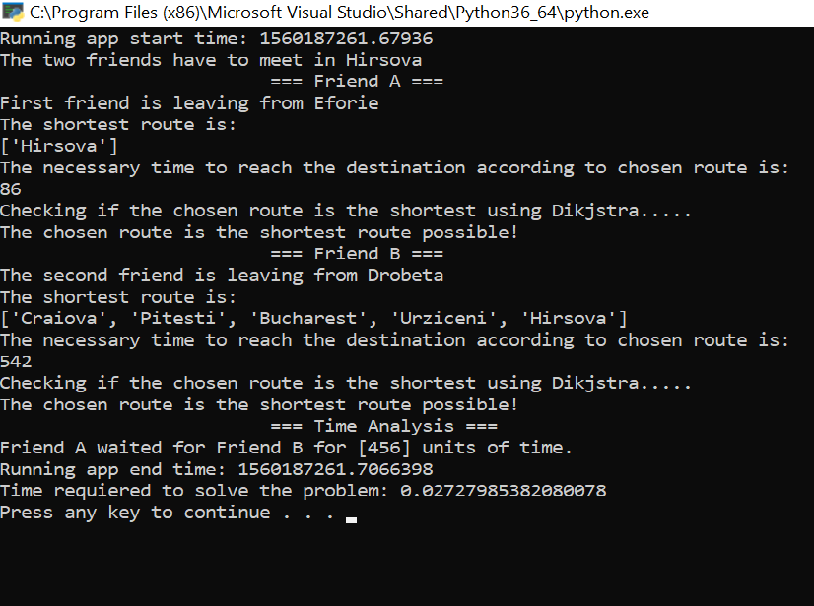
\includegraphics[width=6.3in,height=4.68in]{./media/image4.png}
\end{figure}


%%%%%%%%%%%%%%%%%%%% Figure/Image No: 6 Ends here %%%%%%%%%%%%%%%%%%%%

\begin{itemize}
	\item \par



%%%%%%%%%%%%%%%%%%%% Figure/Image No: 7 starts here %%%%%%%%%%%%%%%%%%%%

\begin{figure}[H]
	\begin{Center}
		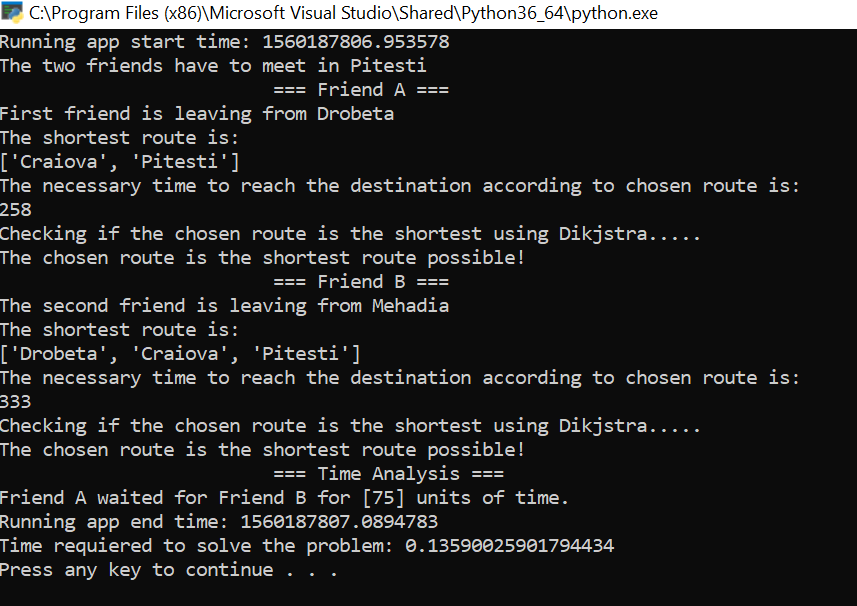
\includegraphics[width=5.55in,height=3.92in]{./media/image9.png}
	\end{Center}
\end{figure}


%%%%%%%%%%%%%%%%%%%% Figure/Image No: 7 Ends here %%%%%%%%%%%%%%%%%%%%

\begin{justify}
 
\end{justify}\par



%%%%%%%%%%%%%%%%%%%% Figure/Image No: 8 starts here %%%%%%%%%%%%%%%%%%%%

\begin{figure}[H]
\advance\leftskip 0.6in		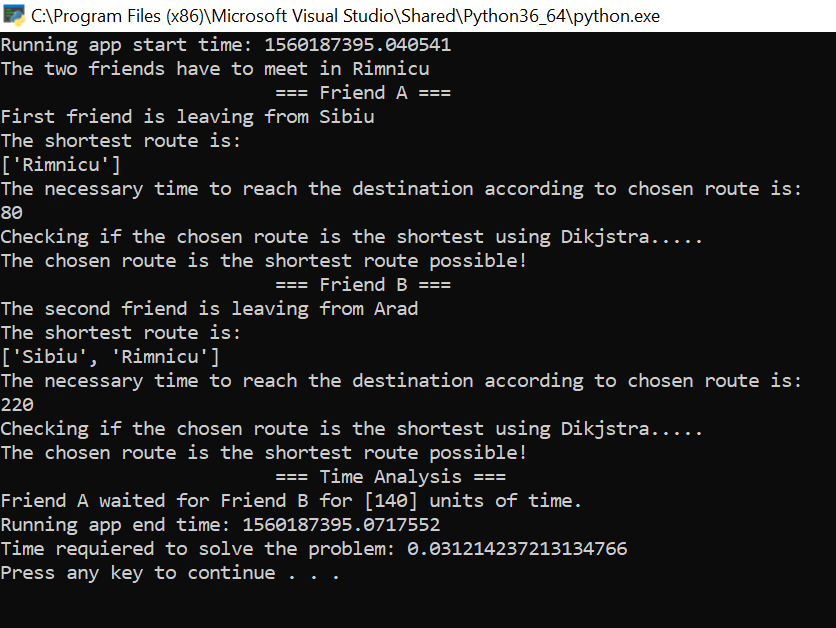
\includegraphics[width=5.73in,height=4.31in]{./media/image15.png}
\end{figure}


%%%%%%%%%%%%%%%%%%%% Figure/Image No: 8 Ends here %%%%%%%%%%%%%%%%%%%%

	\item  \par



%%%%%%%%%%%%%%%%%%%% Figure/Image No: 9 starts here %%%%%%%%%%%%%%%%%%%%

\begin{figure}[H]
	\begin{Center}
		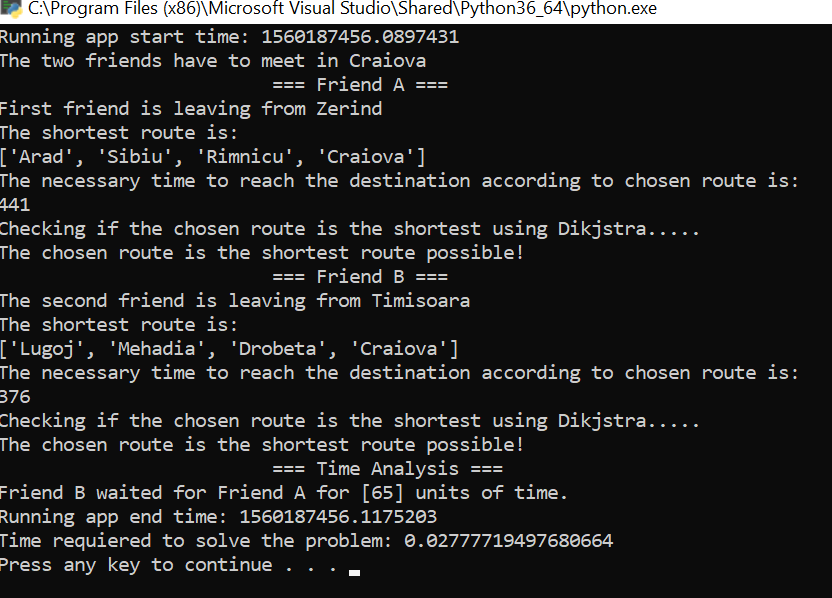
\includegraphics[width=5.63in,height=4.04in]{./media/image3.png}
	\end{Center}
\end{figure}


%%%%%%%%%%%%%%%%%%%% Figure/Image No: 9 Ends here %%%%%%%%%%%%%%%%%%%%

	\item  \par



%%%%%%%%%%%%%%%%%%%% Figure/Image No: 10 starts here %%%%%%%%%%%%%%%%%%%%

\begin{figure}[H]
	\begin{Center}
		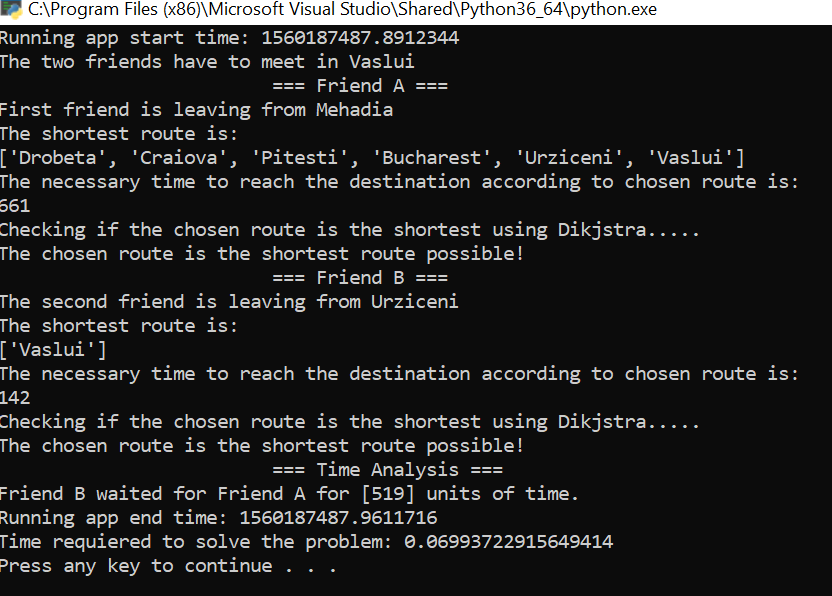
\includegraphics[width=5.67in,height=4.06in]{./media/image16.png}
	\end{Center}
\end{figure}


%%%%%%%%%%%%%%%%%%%% Figure/Image No: 10 Ends here %%%%%%%%%%%%%%%%%%%%

	\item \  \par



%%%%%%%%%%%%%%%%%%%% Figure/Image No: 11 starts here %%%%%%%%%%%%%%%%%%%%

\begin{figure}[H]
	\begin{Center}
		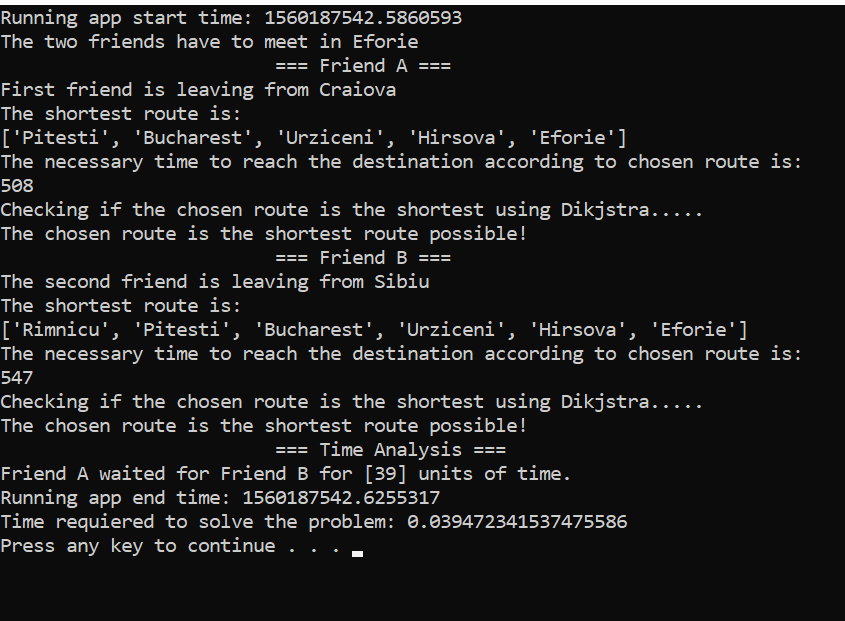
\includegraphics[width=5.61in,height=4.12in]{./media/image7.png}
	\end{Center}
\end{figure}


%%%%%%%%%%%%%%%%%%%% Figure/Image No: 11 Ends here %%%%%%%%%%%%%%%%%%%%

	\item \  \par



%%%%%%%%%%%%%%%%%%%% Figure/Image No: 12 starts here %%%%%%%%%%%%%%%%%%%%

\begin{figure}[H]
	\begin{Center}
		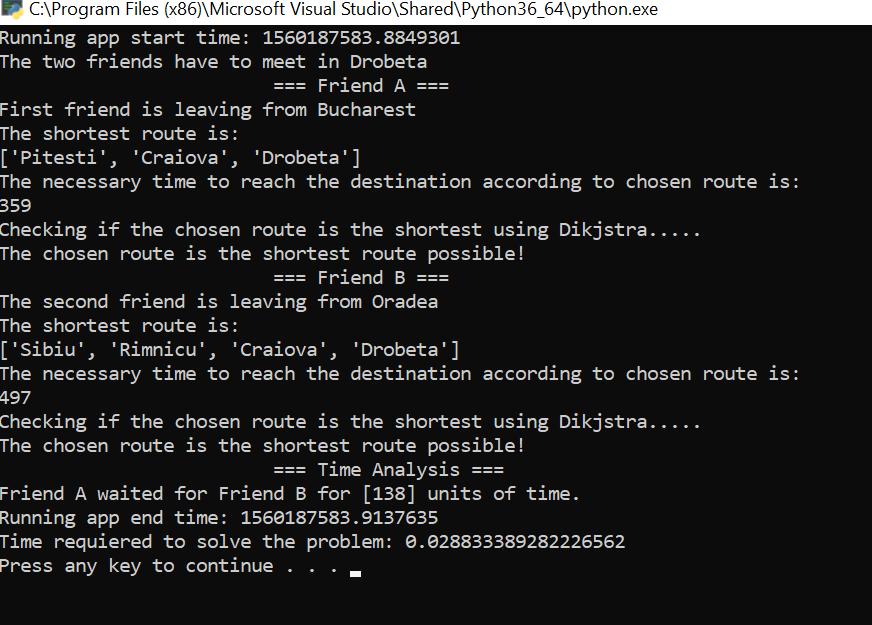
\includegraphics[width=5.61in,height=4.02in]{./media/image14.png}
	\end{Center}
\end{figure}


%%%%%%%%%%%%%%%%%%%% Figure/Image No: 12 Ends here %%%%%%%%%%%%%%%%%%%%

	\item \ \  \par



%%%%%%%%%%%%%%%%%%%% Figure/Image No: 13 starts here %%%%%%%%%%%%%%%%%%%%

\begin{figure}[H]
	\begin{Center}
		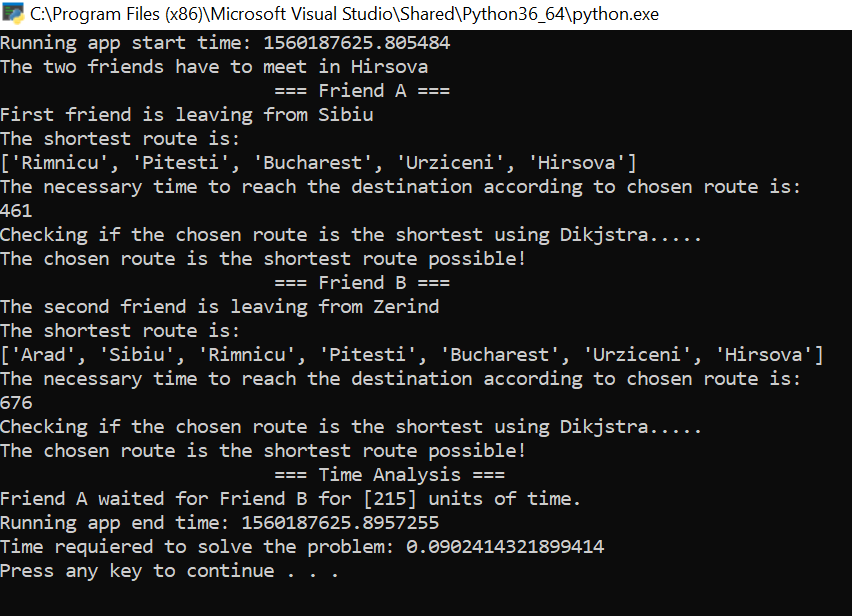
\includegraphics[width=5.66in,height=4.09in]{./media/image2.png}
	\end{Center}
\end{figure}


%%%%%%%%%%%%%%%%%%%% Figure/Image No: 13 Ends here %%%%%%%%%%%%%%%%%%%%

	\item \ \  \par



%%%%%%%%%%%%%%%%%%%% Figure/Image No: 14 starts here %%%%%%%%%%%%%%%%%%%%

\begin{figure}[H]
	\begin{Center}
		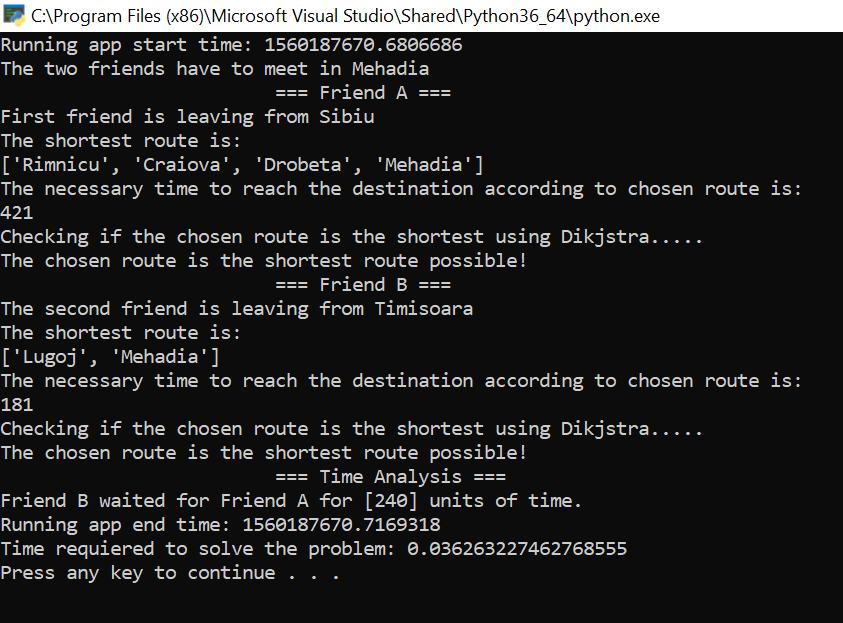
\includegraphics[width=6.05in,height=4.46in]{./media/image6.png}
	\end{Center}
\end{figure}


%%%%%%%%%%%%%%%%%%%% Figure/Image No: 14 Ends here %%%%%%%%%%%%%%%%%%%%

	\item \ \  \par



%%%%%%%%%%%%%%%%%%%% Figure/Image No: 15 starts here %%%%%%%%%%%%%%%%%%%%

\begin{figure}[H]
	\begin{Center}
		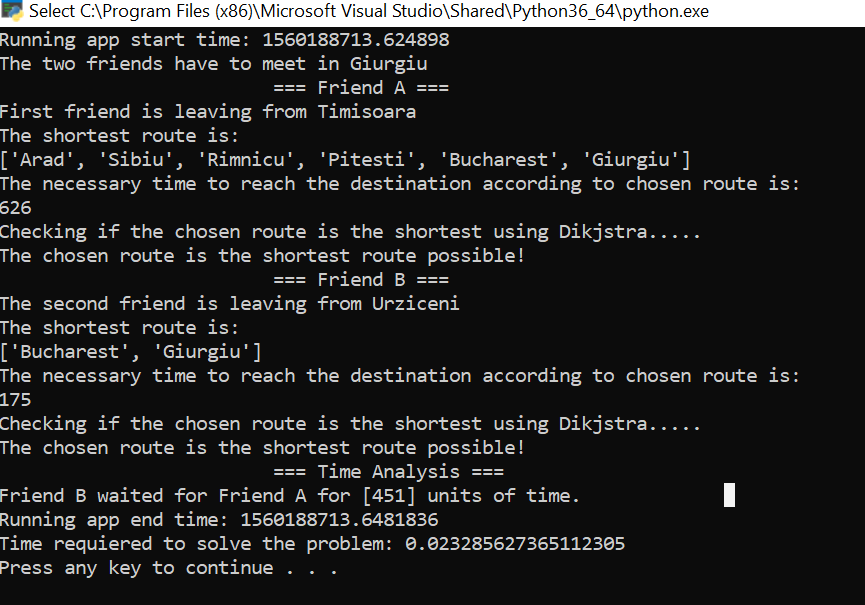
\includegraphics[width=5.82in,height=4.06in]{./media/image5.png}
	\end{Center}
\end{figure}


%%%%%%%%%%%%%%%%%%%% Figure/Image No: 15 Ends here %%%%%%%%%%%%%%%%%%%%

	\item \par



%%%%%%%%%%%%%%%%%%%% Figure/Image No: 16 starts here %%%%%%%%%%%%%%%%%%%%

\begin{figure}[H]
	\begin{Center}
		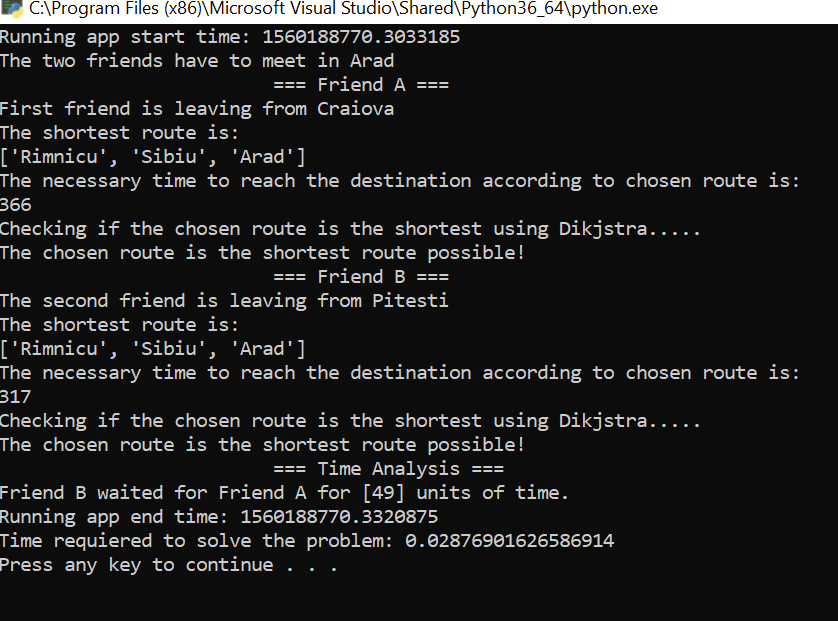
\includegraphics[width=5.51in,height=4.08in]{./media/image8.png}
	\end{Center}
\end{figure}


%%%%%%%%%%%%%%%%%%%% Figure/Image No: 16 Ends here %%%%%%%%%%%%%%%%%%%%

	\item \par



%%%%%%%%%%%%%%%%%%%% Figure/Image No: 17 starts here %%%%%%%%%%%%%%%%%%%%

\begin{figure}[H]
	\begin{Center}
		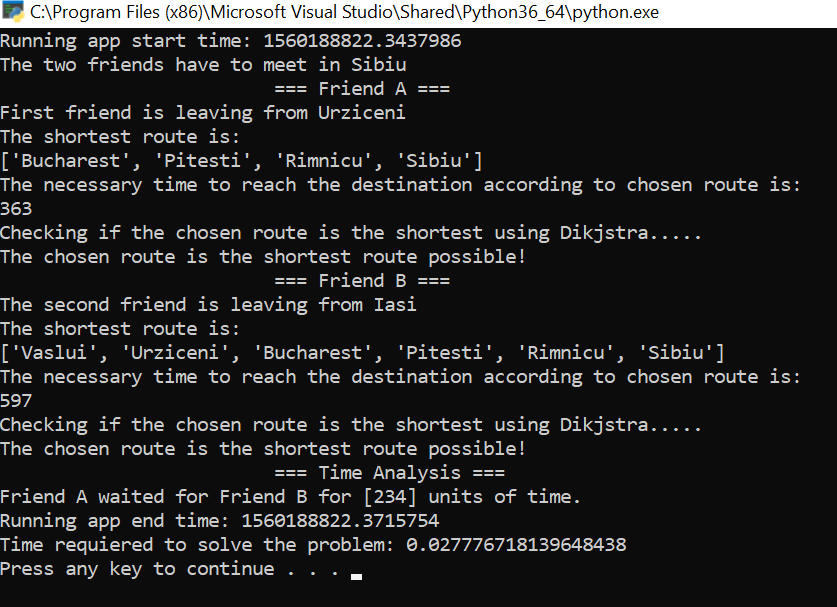
\includegraphics[width=5.72in,height=4.15in]{./media/image10.png}
	\end{Center}
\end{figure}


%%%%%%%%%%%%%%%%%%%% Figure/Image No: 17 Ends here %%%%%%%%%%%%%%%%%%%%

	\item \par



%%%%%%%%%%%%%%%%%%%% Figure/Image No: 18 starts here %%%%%%%%%%%%%%%%%%%%

\begin{figure}[H]
	\begin{Center}
		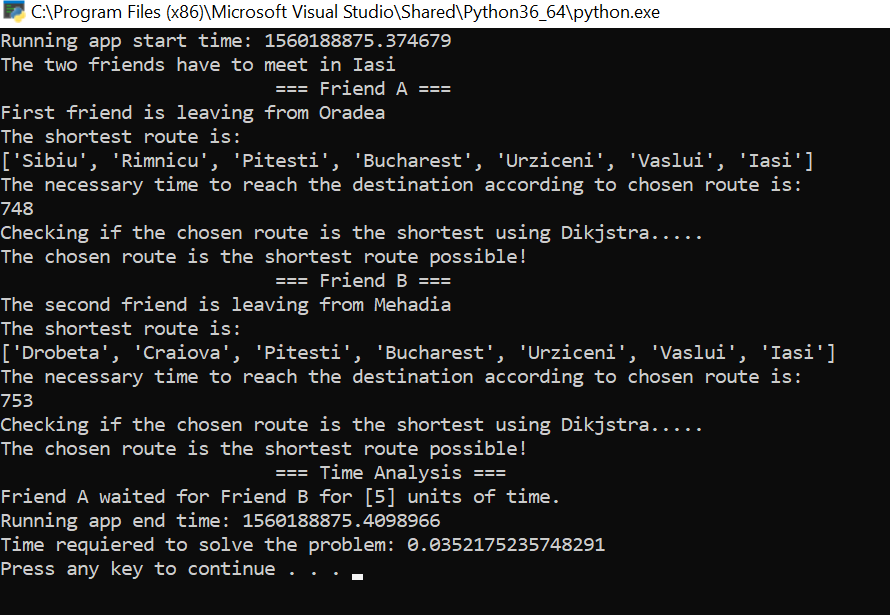
\includegraphics[width=5.59in,height=3.86in]{./media/image17.png}
	\end{Center}
\end{figure}


%%%%%%%%%%%%%%%%%%%% Figure/Image No: 18 Ends here %%%%%%%%%%%%%%%%%%%%

	\item \par


\end{itemize}\section*{Conclusions}
\addcontentsline{toc}{section}{Conclusions}
\begin{justify}
\tab The favourite part of this problem was the practical sense of the statement. Given a real map, with real costs and coordinates, I could solve using heuristic search strategy a practical and perhaps real problem.
\end{justify}\par

\begin{justify}
\tab Some\ improvements can be done regarding the generality of the solution. I used the map of Romania as constant data, but easily I can make this solution also available for any given map, or more precisely for any given cities and the distances between them. As a result, the 2 friends could plan meeting even if they are in different countries. They could be anywhere, as long as they would provide a similar map with cost, the solution described in this project would be available, but with little modifications.  
\end{justify}\par

\begin{justify}
\tab One of my favourite achievements of this project was the organisation of the code, I wanted to create a readable application with clean code organisation. I liked that I could combine the OOP knowledge with the algorithms and strategies used in AI problems. Also, it was a challenge to choose the most friendly and practical way of output such that the result generated is understood as good as possible.
\end{justify}\par


\vspace{\baselineskip}

\printbibliography
\end{document}